% Template for PLoS
% Version 3.1 February 2015
%
% To compile to pdf, run:
% latex plos.template
% bibtex plos.template
% latex plos.template
% latex plos.template
% dvipdf plos.template
%
% % % % % % % % % % % % % % % % % % % % % %
%
% -- IMPORTANT NOTE
%
% This template contains comments intended
% to minimize problems and delays during our production
% process. Please follow the template instructions
% whenever possible.
%
% % % % % % % % % % % % % % % % % % % % % % %
%
% Once your paper is accepted for publication,
% PLEASE REMOVE ALL TRACKED CHANGES in this file and leave only
% the final text of your manuscript.
%
% There are no restrictions on package use within the LaTeX files except that
% no packages listed in the template may be deleted.
%
% Please do not include colors or graphics in the text.
%
% Please do not create a heading level below \subsection. For 3rd level headings, use \paragraph{}.
%
% % % % % % % % % % % % % % % % % % % % % % %
%
% -- FIGURES AND TABLES
%
% Please include tables/figure captions directly after the paragraph where they are first cited in the text.
%
% DO NOT INCLUDE GRAPHICS IN YOUR MANUSCRIPT
% - Figures should be uploaded separately from your manuscript file.
% - Figures generated using LaTeX should be extracted and removed from the PDF before submission.
% - Figures containing multiple panels/subfigures must be combined into one image file before submission.
% For figure citations, please use "Fig." instead of "Figure".
% See http://www.plosone.org/static/figureGuidelines for PLOS figure guidelines.
%
% Tables should be cell-based and may not contain:
% - tabs/spacing/line breaks within cells to alter layout or alignment
% - vertically-merged cells (no tabular environments within tabular environments, do not use \multirow)
% - colors, shading, or graphic objects
% See http://www.plosone.org/static/figureGuidelines#tables for table guidelines.
%
% For tables that exceed the width of the text column, use the adjustwidth environment as illustrated in the example table in text below.
%
% % % % % % % % % % % % % % % % % % % % % % % %
%
% -- EQUATIONS, MATH SYMBOLS, SUBSCRIPTS, AND SUPERSCRIPTS
%
% IMPORTANT
% Below are a few tips to help format your equations and other special characters according to our specifications. For more tips to help reduce the possibility of formatting errors during conversion, please see our LaTeX guidelines at http://www.plosone.org/static/latexGuidelines
%
% Please be sure to include all portions of an equation in the math environment.
%
% Do not include text that is not math in the math environment. For example, CO2 will be CO\textsubscript{2}.
%
% Please add line breaks to long display equations when possible in order to fit size of the column.
%
% For inline equations, please do not include punctuation (commas, etc) within the math environment unless this is part of the equation.
%
% % % % % % % % % % % % % % % % % % % % % % % %
%
% Please contact latex@plos.org with any questions.
%
% % % % % % % % % % % % % % % % % % % % % % % %

\documentclass[10pt,letterpaper]{article}
\usepackage[top=0.85in,left=2.75in,footskip=0.75in]{geometry}

% Use adjustwidth environment to exceed column width (see example table in text)
\usepackage{changepage}

% Use Unicode characters when possible
\usepackage[utf8]{inputenc}

% textcomp package and marvosym package for additional characters
\usepackage{textcomp,marvosym}

% fixltx2e package for \textsubscript
\usepackage{fixltx2e}

% amsmath and amssymb packages, useful for mathematical formulas and symbols
\usepackage{amsmath,amssymb}

% cite package, to clean up citations in the main text. Do not remove.
\usepackage{cite}

% Use nameref to cite supporting information files (see Supporting Information section for more info)
\usepackage{nameref,hyperref}

% line numbers
\usepackage[right]{lineno}

% ligatures disabled
\usepackage{microtype}
%\DisableLigatures[f]{encoding = *, family = * }

% rotating package for sideways tables
\usepackage{rotating}

\usepackage{tikz}
\usepackage{subfig}
\usepackage{algorithm}
\usepackage{algpseudocode}
\usepackage{calc}
\usepackage{siunitx}
%\usepackage{graphics}
\graphicspath{{figures/upload/}}  % added by JMP


% Remove comment for double spacing
%\usepackage{setspace}
%\doublespacing

% Text layout
\raggedright
\setlength{\parindent}{0.5cm}
\textwidth 5.25in
\textheight 8.75in

% Bold the 'Figure #' in the caption and separate it from the title/caption with a period
% Captions will be left justified
\usepackage[aboveskip=1pt,labelfont=bf,labelsep=period,justification=raggedright,singlelinecheck=off]{caption}

% Use the PLoS provided BiBTeX style
\bibliographystyle{plos2015}

% Remove brackets from numbering in List of References
\makeatletter
\renewcommand{\@biblabel}[1]{\quad#1.}
\makeatother

% Leave date blank
\date{}

% Header and Footer with logo
\usepackage{lastpage,fancyhdr,graphicx}
\usepackage{epstopdf}
\pagestyle{myheadings}
\pagestyle{fancy}
\fancyhf{}
%\lhead{
\includegraphics[width=2.0in]{PLOS-submission.eps}}
\fancyhead[R]{\fontsize{12}{14} \selectfont Neuron's Eye View: Inferring Features of Complex Stimuli from Neural Responses}
\rfoot{\thepage/\pageref{LastPage}}
\renewcommand{\footrule}{\hrule height 2pt \vspace{2mm}}
\fancyheadoffset[L]{2.25in}
\fancyfootoffset[L]{2.25in}
\lfoot{\sf PLOS}

%% Include all macros below

\newcommand{\lorem}{{\bf LOREM}}
\newcommand{\ipsum}{{\bf IPSUM}}

% Generelt
\newcommand{\ud}{\mathrm{d}} % d
\newcommand{\R}{\mathbb{R}} % Real numbers
\newcommand{\T}{\mathscr{T}}

% Operatorer og funktionaler
\newcommand{\I}{\mathbb{I}} % I

\newcommand{\CE}[2]{\mathrm{E}\left[\,#1\,|\,#2\,\right]} % Conditional expectation

\newcommand{\by}{\boldsymbol{y}}
\newcommand{\bc}{\boldsymbol{c}}
\newcommand{\bd}{\boldsymbol{d}}
\newcommand{\bP}{\boldsymbol{\Phi}}
\newcommand{\bZ}{Z}%{\boldsymbol{Z}}
\newcommand{\bV}{V}%{\boldsymbol{V}}
\newcommand{\br}{\boldsymbol{r}}
\newcommand{\bt}{\boldsymbol{t}}
\newcommand{\btheta}{\boldsymbol{\vartheta}}
\newcommand{\bht}{\hat{\boldsymbol{\vartheta}}}
\newcommand{\bz}{\boldsymbol{z}}
\newcommand{\bx}{{\boldsymbol{x}}}
\newcommand{\bv}{v}
\newcommand{\bw}{\boldsymbol{w}}
\newcommand{\vv}{\boldsymbol{v}}
\newcommand{\bepsilon}{\boldsymbol{\varepsilon}}

%% END MACROS SECTION

\setcounter{secnumdepth}{3}
\begin{document}
\vspace*{0.35in}

% Title must be 250 characters or less.
% Please capitalize all terms in the title except conjunctions, prepositions, and articles.
\begin{flushleft}
{\Large
\textbf{S2 Text. Inferred latents as classification features\\}
\bigskip
% \textbf{Inferred latents as classification features} % Please use "title case" (capitalize all terms in the title except conjunctions, prepositions, and articles).
}
% \newline
% % Insert author names, affiliations and corresponding author email (do not include titles, positions, or degrees).
% Xin (Cindy) Chen\textsuperscript{1,3},
% Jeffrey M. Beck\textsuperscript{2,3},
% John M. Pearson\textsuperscript{1,3*},
% \\
% \bigskip
% \textbf{1} Duke Institute for Brain Sciences, Duke University, Durham, North Carolina, USA
% \\
% \textbf{2} Department of Neurobiology, Duke University Medical Center, Durham, North Carolina, USA
% \\
% \textbf{3} Center for Cognitive Neuroscience, Duke University, Durham, North Carolina, USA
% \\

% Insert additional author notes using the symbols described below. Insert symbol callouts after author names as necessary.
%
% Remove or comment out the author notes below if they aren't used.
%
% Primary Equal Contribution Note
%\Yinyang These authors contributed equally to this work.

% Deceased author note
%\dag Deceased

% Group/Consortium Author Note
%\textpilcrow Membership list can be found in the Acknowledgments section.

% Use the asterisk to denote corresponding authorship and provide email address in note below.
% * john.pearson@duke.edu

\end{flushleft}
% Please keep the abstract below 300 words

% Place figure captions after the first paragraph in which they are cited.

As a byproduct of our model, the generated labels provide a concise and fairly complete summary of the stimulus-related activity in the neural recordings. Here we want to emphasize that although our model is not a data compression method, it nonetheless preserves most of the information from raw data.

Here, we use all pairwise combinations of binary features of our model to train a sparse logistic regression predicting stimulus category. We compare the results of this to a multinomial logistic regression on raw spike counts with L1 and L2 regularization. Results are shown in Figure \ref{fig:softmax}.

\begin{figure}[!ht]
    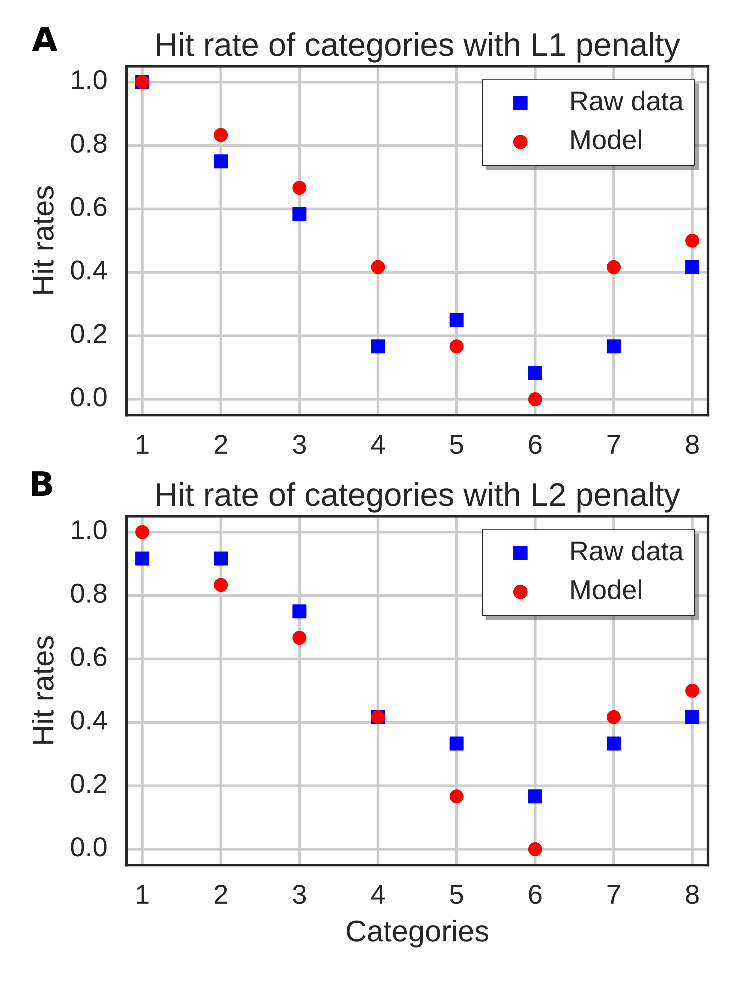
\includegraphics[width=.7\linewidth]{softmax}
	\caption{\bf Comparison of actual and inferred states of the macaque dataset.}
    A. The overall hit rate of prediction with L1 regularization respect to eight categories: Faces, Animals, Bodies, Fruit, Natural, Manmade, Scene, Pattern. B. The overall hit rate of prediction with L1 regularization for eight categories.
	 %using raw data and inferred features for visual category dataset.
	\label{fig:softmax}
\end{figure}


\end{document}
